\section{Data Analysis}
\label{Data Analysis}

\subsection{Vertical Radiation Profile}
\begin{figure}[H]
\centering
\begin{subfigure}{.5\textwidth}
  \centering
  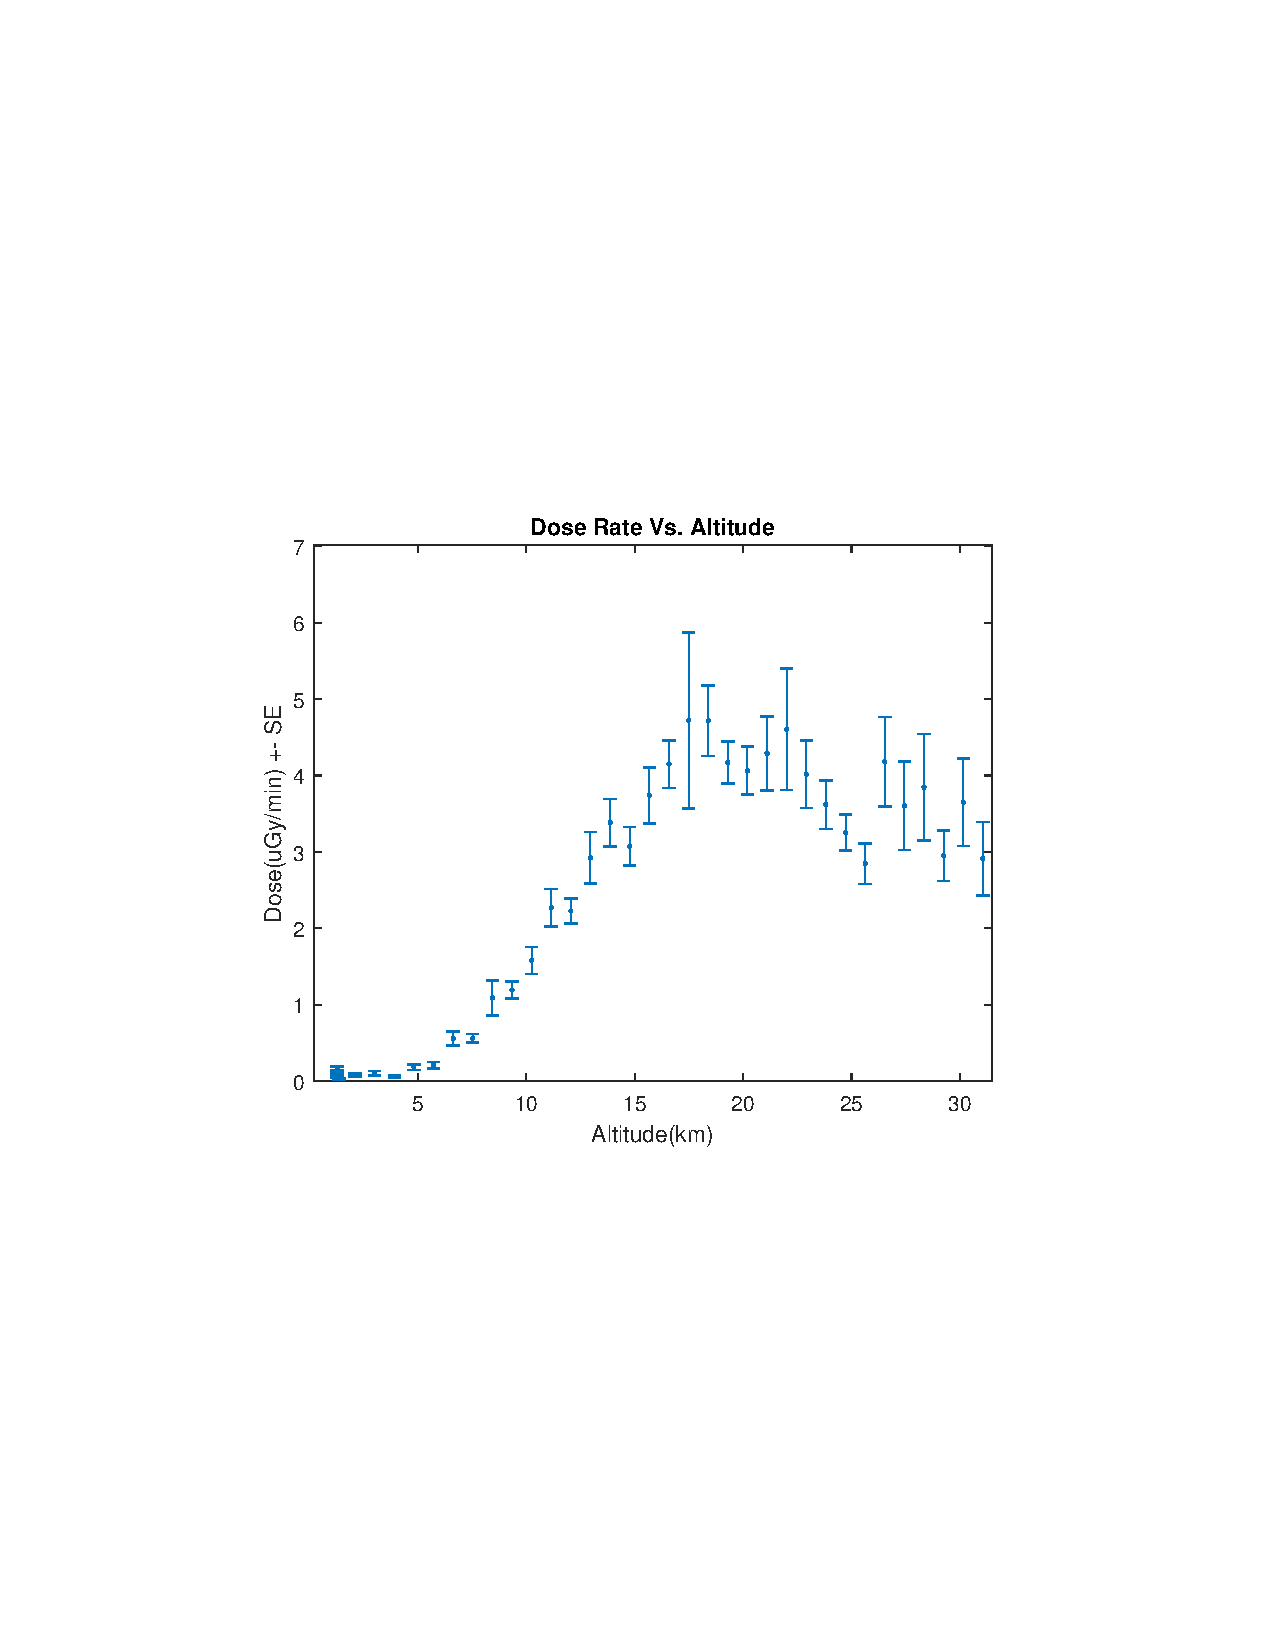
\includegraphics[scale=.5]{doseerror_cropped.pdf}
  \caption{Dose rate in silicon vs. altitude.}
  \label{fig:sub1}
\end{subfigure}%
\begin{subfigure}{.5\textwidth}
  \centering
  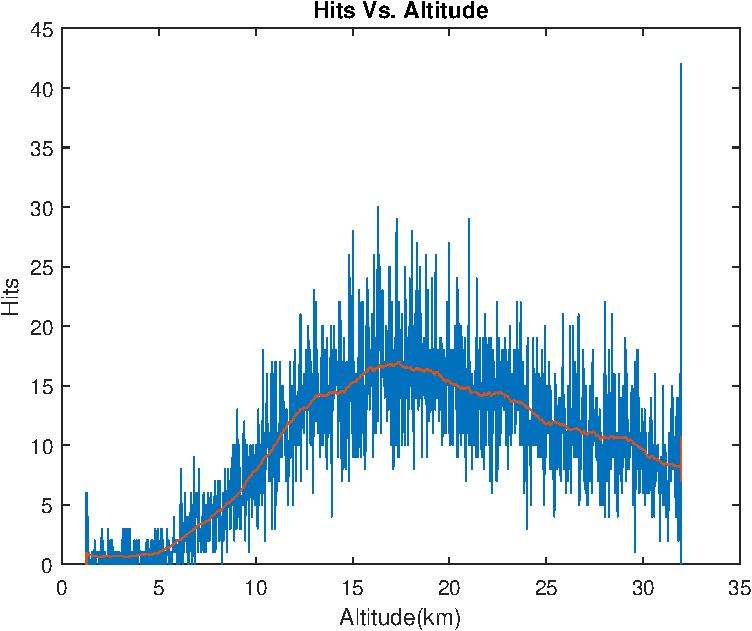
\includegraphics[scale=.5]{hva-cropped.pdf}
  \caption{Detector Hits vs. altitude.}
  \label{fig:sub2}
\end{subfigure}
\caption{Not sure what to put here yet.}
\label{fig:test}
\end{figure}

\begin{figure}[H]
\centering
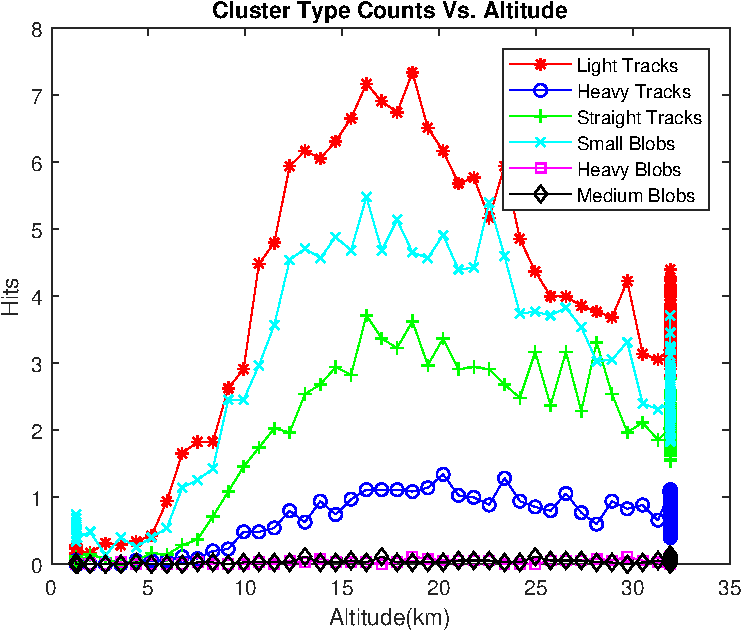
\includegraphics[scale=.5]{ctva-cropped.pdf}
\caption{Cluster Type Counts vs. altitude.}
\end{figure}

\begin{figure}[H]
\centering
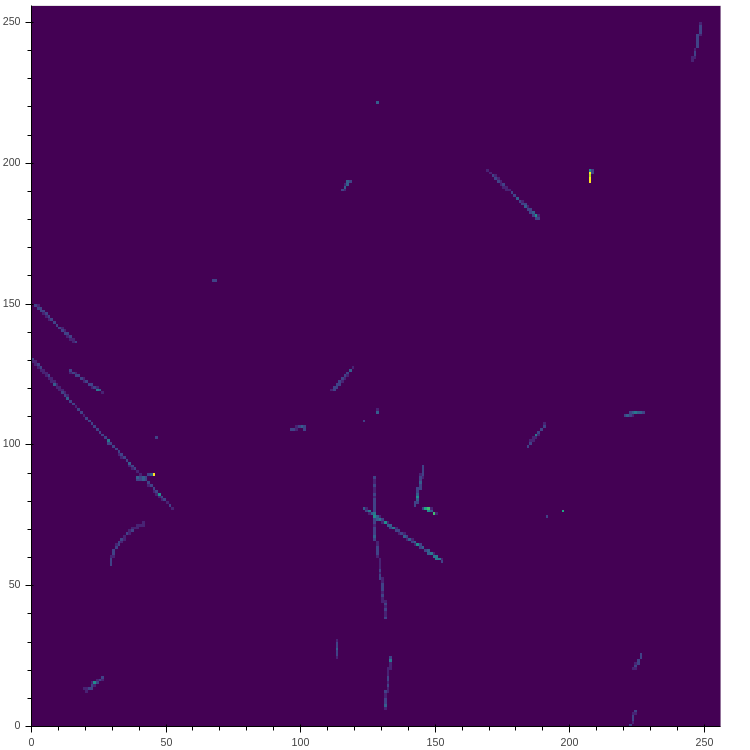
\includegraphics[scale=.25]{viridis.png}
\caption{Frame collected at float.}
\end{figure}
